\documentclass[12pt]{article}
\usepackage[utf8]{inputenc}
\usepackage[T1]{fontenc}
\usepackage[polish]{babel}
\usepackage{geometry}
\usepackage{tabularx}
\usepackage[table,xcdraw,dvipsnames]{xcolor}
\usepackage{color}
\usepackage{subfig}
\usepackage{sidecap}
\usepackage{wrapfig}
\usepackage{float}
\usepackage{enumerate}
\usepackage{graphicx}
\usepackage{multirow}
\usepackage{hyperref}
\usepackage{titlesec}
\usepackage{amsmath}
\usepackage{anyfontsize}
\usepackage{indentfirst}
\usepackage{listings}
\usepackage{multicol}
\usepackage{pgfplots}
\usepackage{fancyhdr}

\newgeometry{tmargin=1.8cm,bmargin=1.8cm,lmargin =1.8cm,rmargin=1.8cm}

\begin{document}
\begin{titlepage}
\begin{figure}
    \centering
    
\includegraphics[width=18cm]{logo-PWr.png}
    \label{fig:pwr}
\end{figure}
    \begin{center}
        \LARGE \textbf{ Wydział Elektroniki, Fotoniki i Mikrosystemów }\\ 
        \vspace{70pt}
        \Huge \textit{ Sterowanie Procesami Ciągłymi}  \\
    \end{center}
    \vspace{30pt}
    \hrule
    \vspace{1pt}
    \hrule
    \begin{center}
        {\fontsize{30}{50}\selectfont Sprawozdanie nr 1\\ }
        \vspace{10pt}
        {\fontsize{25}{25}\selectfont Charakterystyki czasowe  }
    \end{center}
    \hrule
    \vspace{1pt}
    \hrule
    \begin{flushright}
        \vspace{50pt}

        \textit{\Large Prowadzący:}\\
        \Large dr hab. inż. Grzegorz Mzyk\\
        \vspace{10pt}
        \textit{\Large Wykonała:}\\
        \Large Zuzanna Mejer, 259382 \\
        \vspace{10pt}
        \textit{\Large Termin zajęć:}\\
        \Large czwartek TP, 9:15\\
        \vspace{10pt}
    
    \end{flushright}
    \vspace{60pt}
    \begin{center}
        \large Wrocław, \today r.
    \end{center}
\end{titlepage}
    
    
\tableofcontents
\newpage

\section{Cel ćwiczenia}
Głównymi celami ćwiczenia było: zbadanie zależności odpowiedzi systemu w dziedzinie czasu od pulsacji pobudzenia sinusoidalnego; zapoznanie się z różnymi rodzajami charakterystyk częstotliwościowych oraz zbadanie wpływu wartości parametrów układu opóźniającego z inercją na charakterystykę częstotliwościową układu.


\section{Zależność charakterystyki czasowej układu od wartości pulsacji pobudzenia sinusoidalnego}
Badany jest asymptotycznie stabilny układ liniowy o zadanej transmitancji:
\begin{equation}
    K(s) = \frac{1}{s^2+0,1s+1},
    \label{transmitancja}
\end{equation}
który pobudzany jest sygnałem sinusoidalnym o ogólnym wzorze:

\begin{equation}
    u(t) = sin(\omega t),
\end{equation}
gdzie $\omega$ to pulsacja. Odpowiedź układu liniowego na pobudzenie sinusoidalne w stanie ustalonym ma postać:
\begin{equation}
    y_{ust}(t) = A \cdot sin(\omega t + \varphi),
\end{equation}
gdzie: $A$ to amplituda, $\omega$ to pulsacja oraz $\varphi$ to przesunięcie fazowe. Wiedząc, że pulsacja odpowiedzi systemu $\omega$ jest identyczna jak pulsacja sygnału wejściowego, zbadano jaka jest zależność między pulsacją sygnału wejściowego a amplitudą $A$ i przesunięciem fazowym $\varphi$ odpowiedzi systemu. Do badań przyjęto 3 wartości pulsacji: $\omega = 0,1$, $\omega = 1$, $\omega = 10$, co oznacza, że układ o transmitancji \ref{transmitancja} pobudzono kolejno: $u_1(t) = sin(0,1t)$, $u_2(t) = sin(1t)$ oraz $u_3(t) = sin(10t)$.  Zbudowano następujący schemat w Simulinku:
\begin{figure}[H]
    \centering
    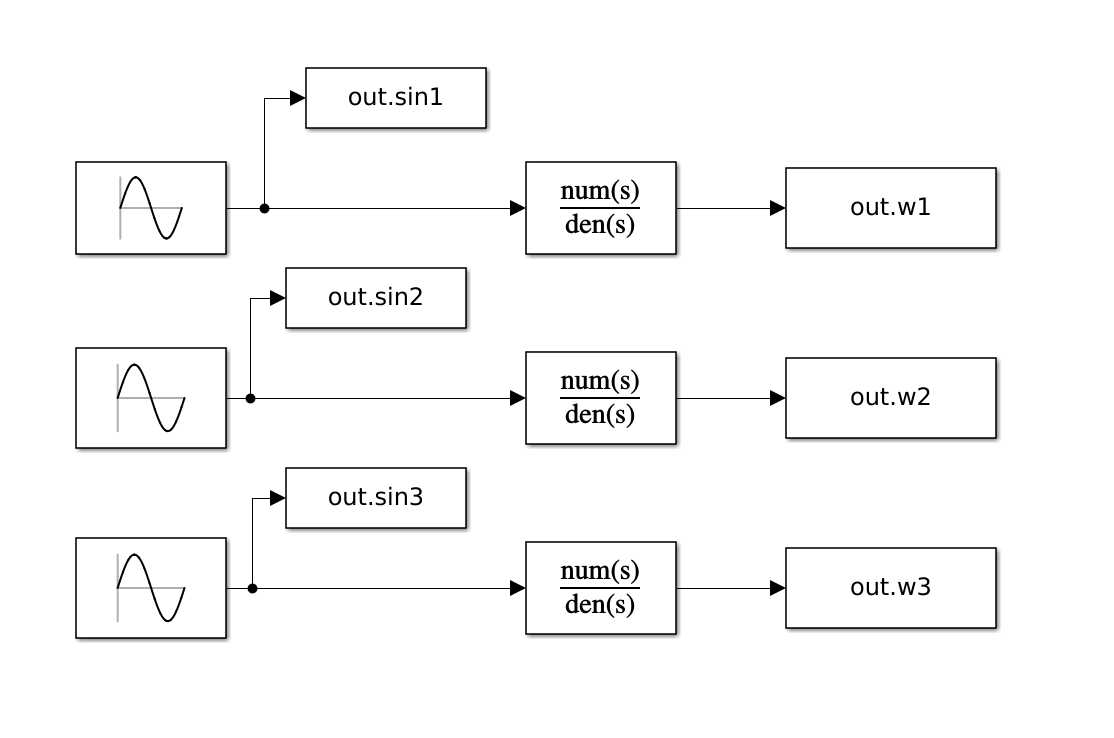
\includegraphics[scale=0.25]{2.png}
    \caption{Schemat w Simulinku do badania odpowiedzi układu na pobudzenie sinusoidalne}
\end{figure}


\subsection{Odpowiedź systemu na pobudzenie sinusoidalne, gdy pulsacja $\omega = 0,1$}
Pobudzono układ sygnałem $u_1(t)=sin(0,1 t)$. Poniżej przedstawiono porównanie pobudzenia sinusoidalnego (kolor czarny na wykresie) z odpowiedzią systemu (kolor czerwony na wykresie).
\begin{figure}[H]
    \centering
    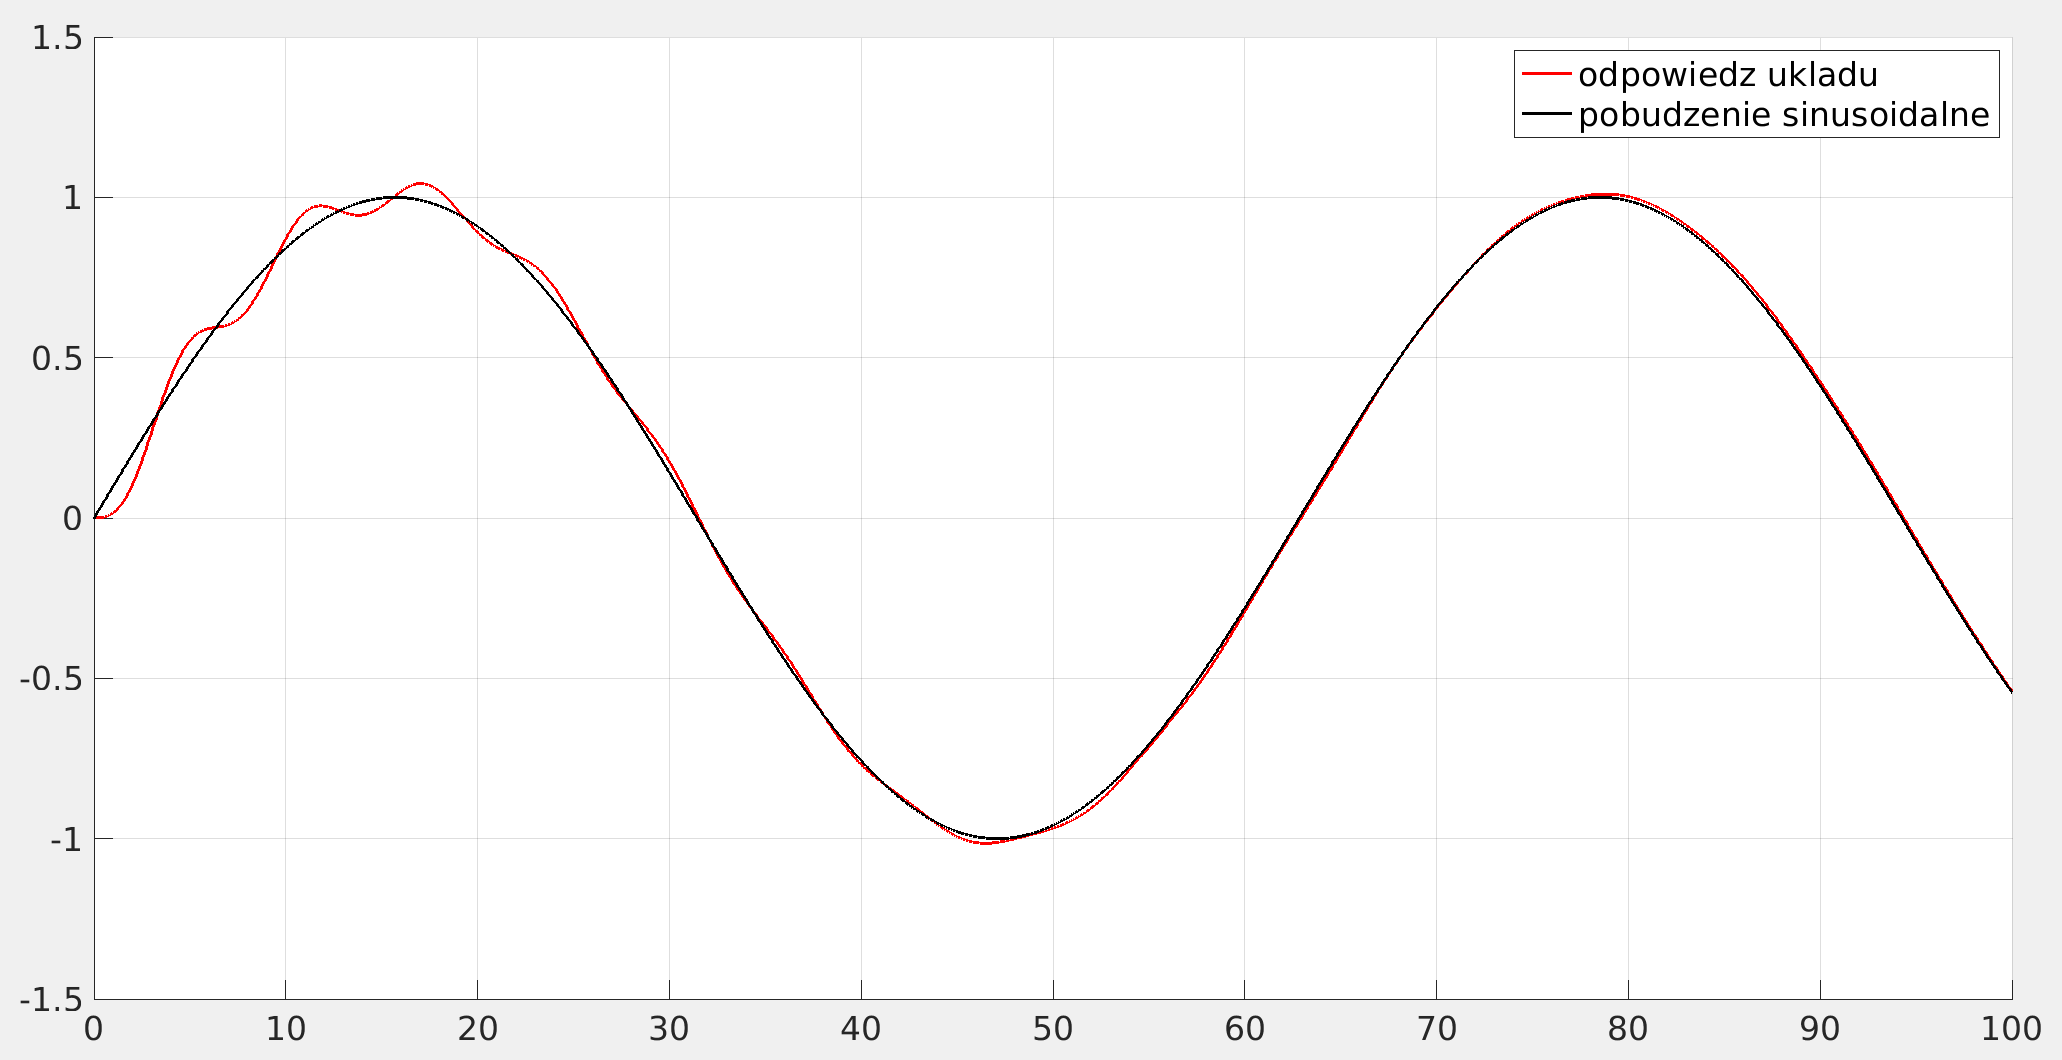
\includegraphics[scale=0.2]{2.1.png}
    \caption{Odpowiedź systemu o transmitancji K(s) na pobudzenie $u_1(t)=sin(0,1 t)$}
\end{figure}

Odpowiedź układu prawie idealnie pokrywa się z pobudzeniem sinusoidalnym. Amplituda wynosi $A=1$ oraz nie ma przesunięcia fazowego $ \varphi=0$.

\subsection{Odpowiedź systemu na pobudzenie sinusoidalne, gdy pulsacja $\omega = 1$}
Pobudzono układ sygnałem $u_2(t)=sin(1 t)$. Poniżej przedstawiono porównanie pobudzenia sinusoidalnego (kolor czarny na wykresie) z odpowiedzią systemu (kolor czerwony na wykresie).
\begin{figure}[H]
    \centering
    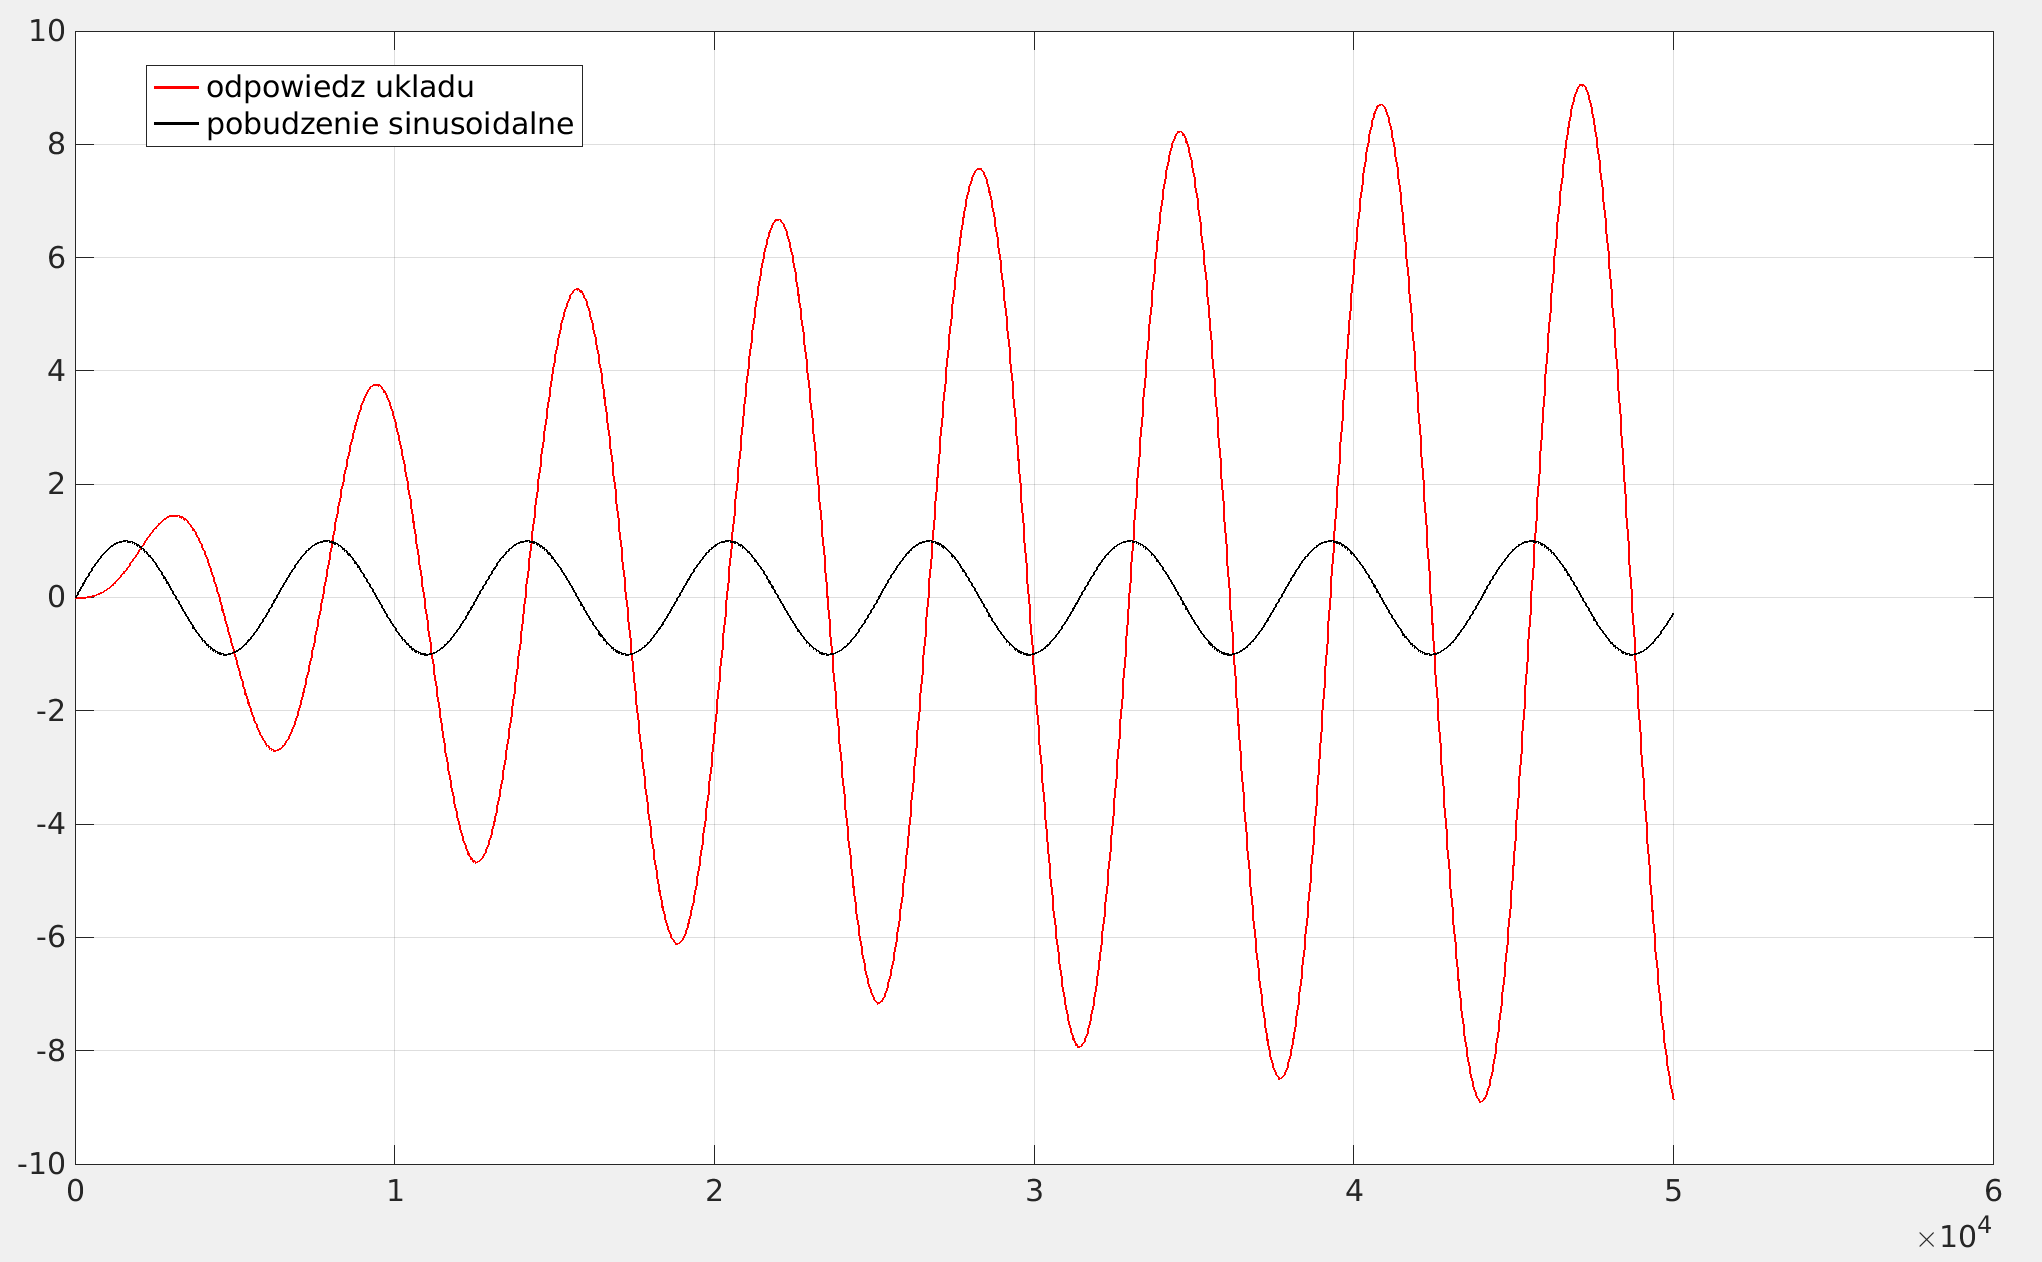
\includegraphics[scale=0.2]{2.2.png}
    \caption{Odpowiedź systemu o transmitancji K(s) na pobudzenie $u_2(t)=sin(1 t)$}
    \label{fig:2}
\end{figure}

Na Rysunku \ref{fig:2} przedstawiony został fragment odpowiedzi układu. Widać na nim, że amplituda odpowiedzi układu wzrasta. Stabilizuje się znacznie później na wartości $A \approx 10$, co przedstawia Rysunek \ref{fig:2.22}:
\begin{figure}[H]
    \centering
    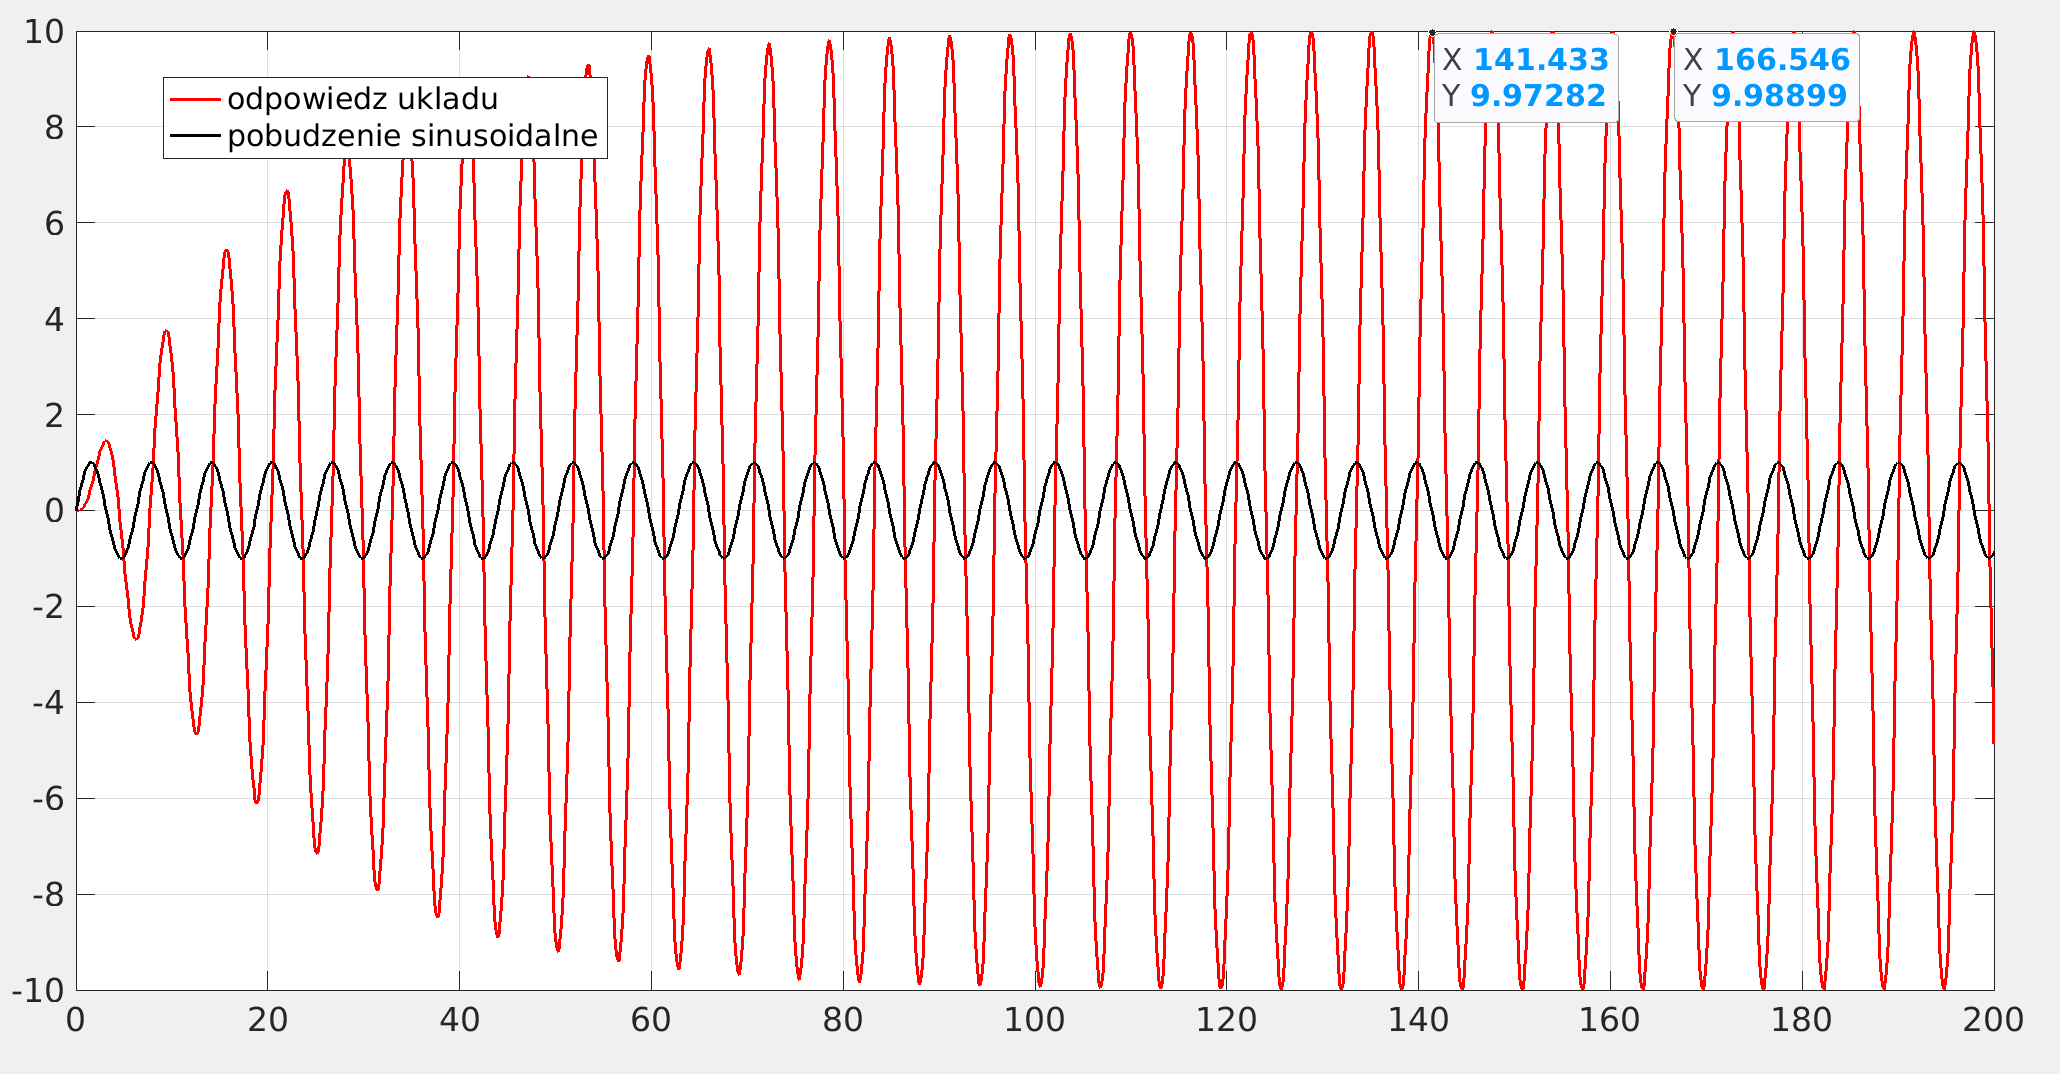
\includegraphics[scale=0.2]{2.22.png}
    \caption{Amplituda odpowiedzi systemu wynosi 10}
    \label{fig:2.22}
\end{figure}

Ze względu na to, że osie na wykresie są w dziedzinie czasu, nie można bezpośrednio odczytać przesunięcia fazowego. Aby wyznaczyć przesunięcie fazowe można skorzystać ze wzoru:
\begin{equation}
    \varphi = \frac{2 \pi}{T} \cdot \tau.
\end{equation}
Wiedząc, że: $\frac{2 \pi}{T} = \omega$, można zapisać ten wzór w postaci:
\begin{equation}
    \varphi = \omega \cdot \tau,
\end{equation}
gdzie $\tau$ to różnica wartości przecięć funkcji z osią $x$, czyli $\tau = x_2 - x_1$. Na Rysunku \ref{fig:2.23} wybrano punkty przecięcia dwóch funkcji z osią $x$. Z Rysunku można odczytać, że: $x_2 = 17,24$ oraz $x_1 = 15,762$. Ponadto, do wzoru potrzebna jest pulsacja, która jest zadana: $\omega = 1$. 
\begin{figure}[H]
    \centering
    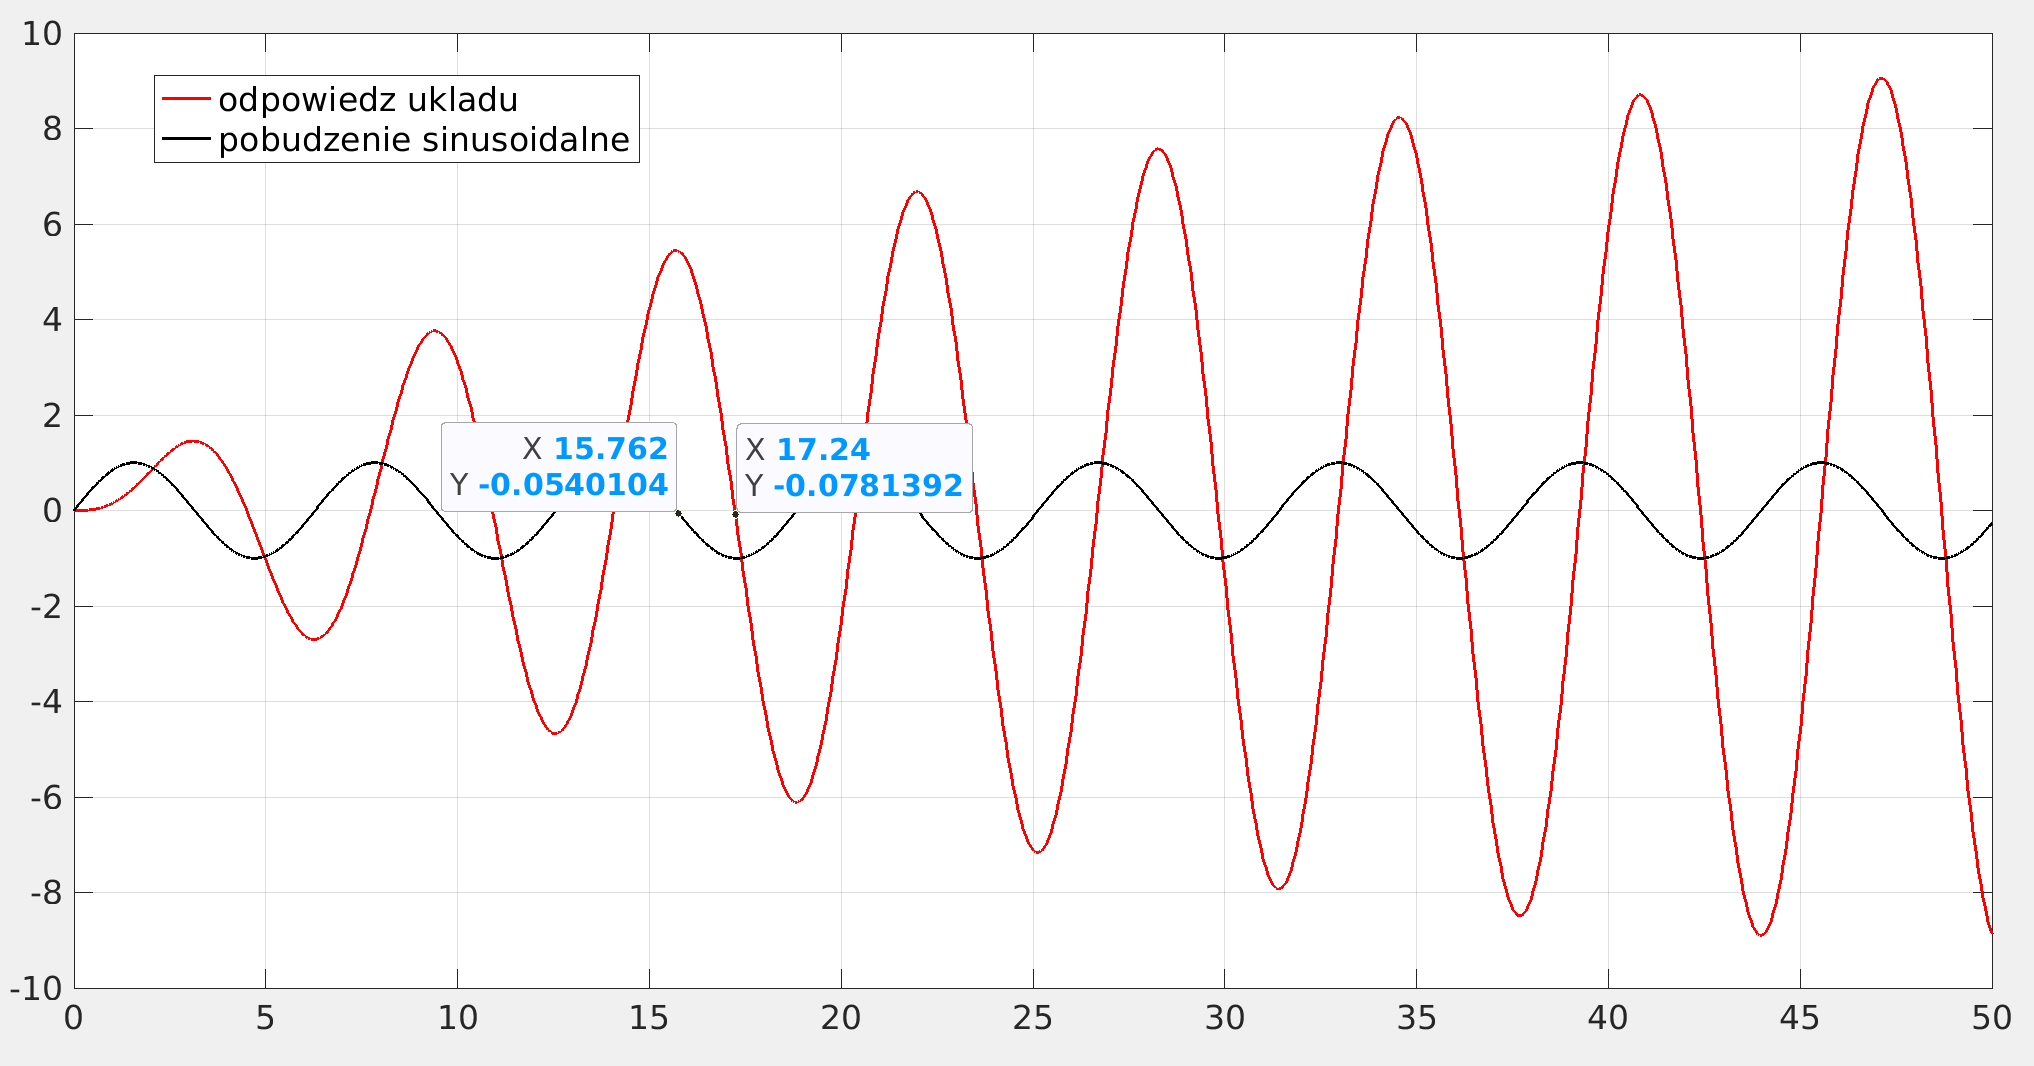
\includegraphics[scale=0.2]{2.23.png}
    \caption{Dane do wyznaczenia przesunięcia fazowego}
    \label{fig:2.23}
\end{figure}
Zatem:
\begin{equation}
    \varphi = 1 \frac{rad}{s} \cdot (17,24 s-15,762s) = 1,478 rad \approx 84,68 ^\circ
\end{equation}
Przesunięcie fazowe między pobudzeniem a odpowiedzią układu wynosi $\varphi \approx 84,68 ^\circ$.

\subsection{Odpowiedź systemu na pobudzenie sinusoidalne, gdy pulsacja $\omega = 10$}
Pobudzono układ sygnałem $u_3(t)=sin(10 t)$. Poniżej przedstawiono porównanie pobudzenia sinusoidalnego (kolor czarny na wykresie) z odpowiedzią systemu (kolor czerwony na wykresie).
\begin{figure}[H]
    \centering
    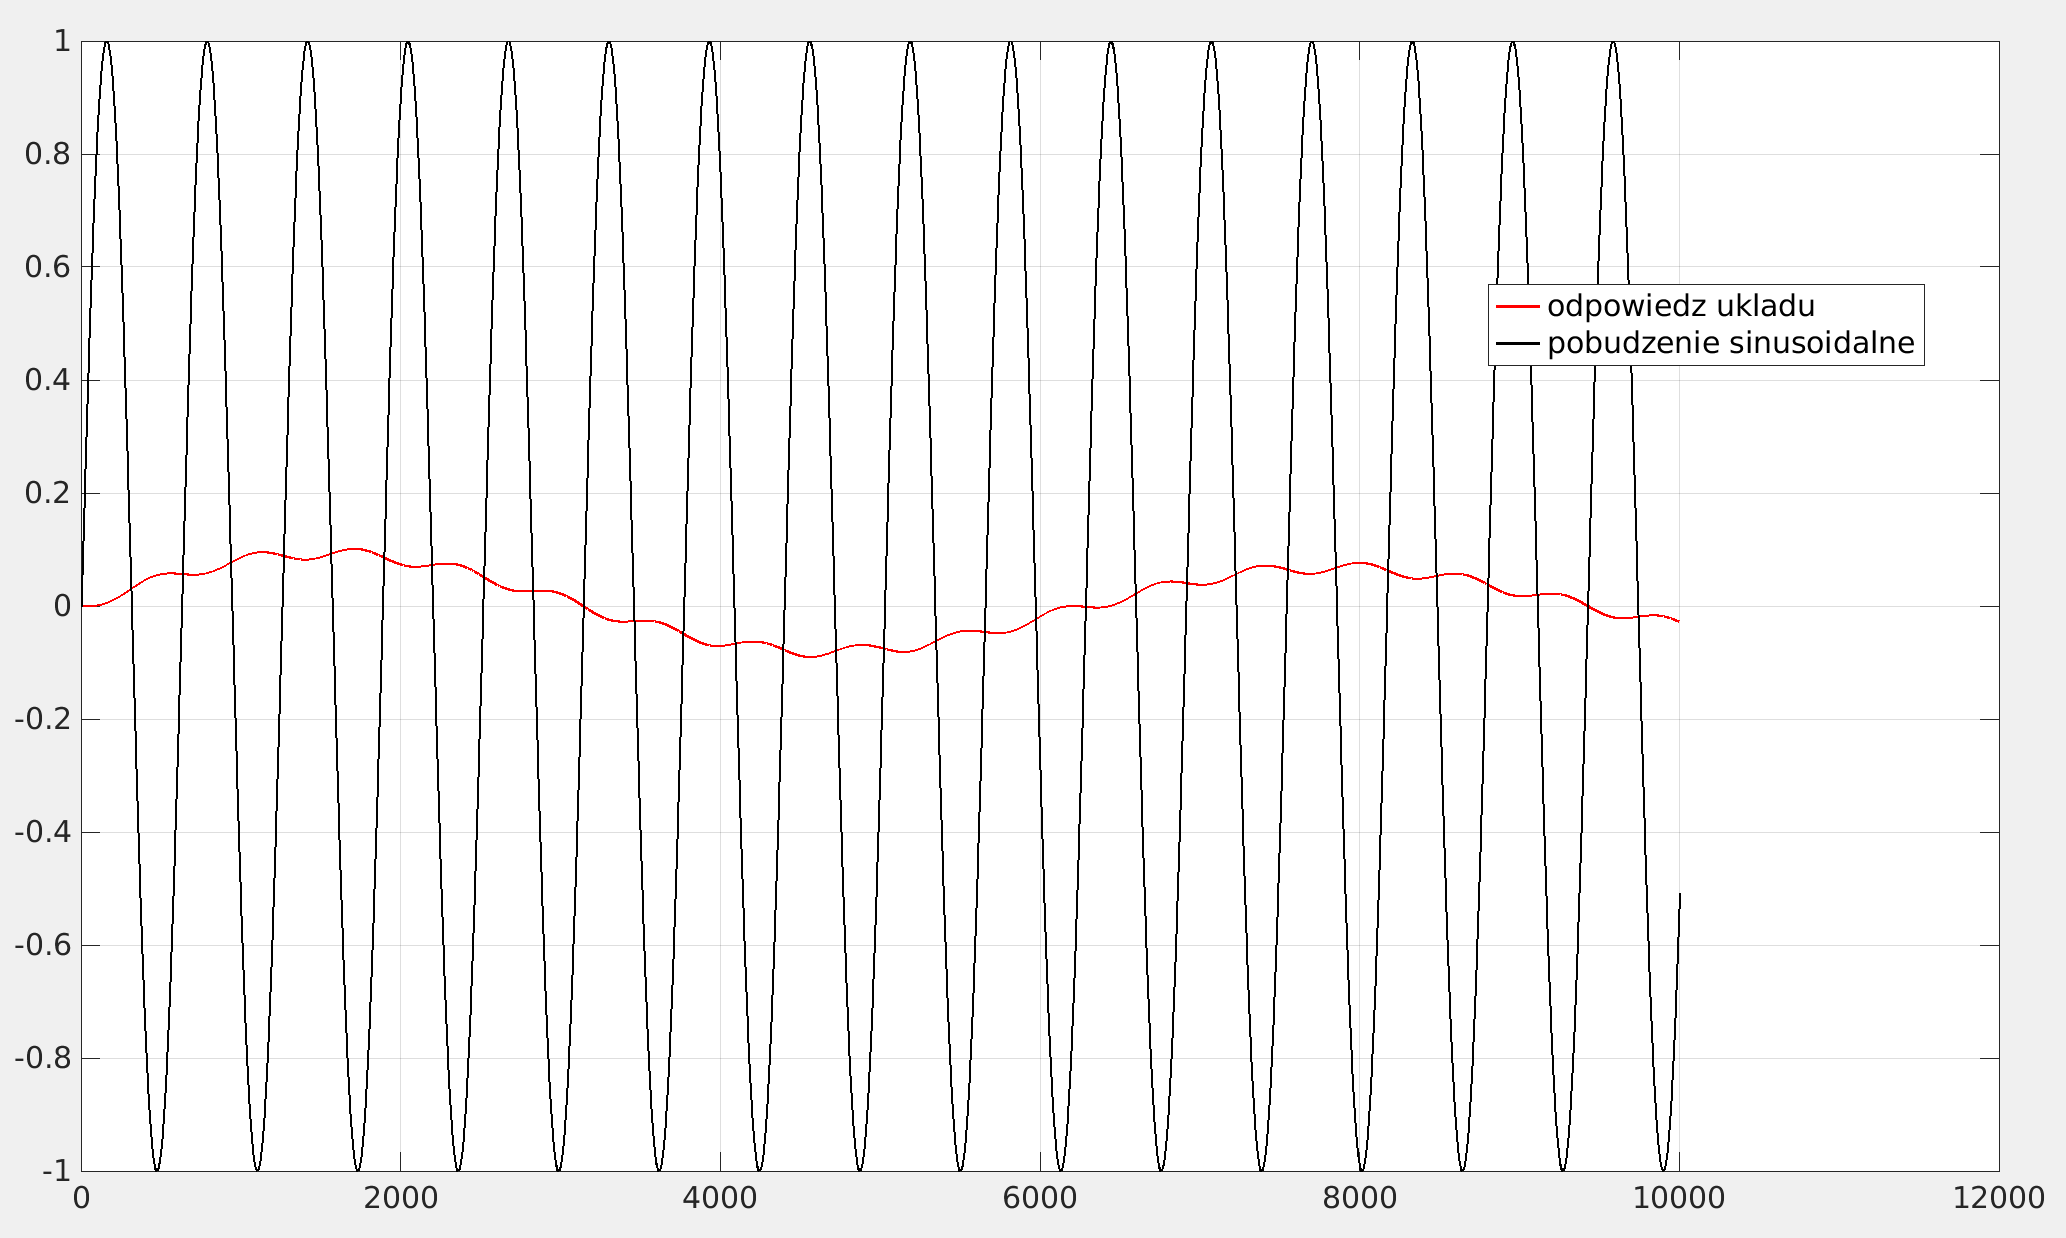
\includegraphics[scale=0.2]{2.3.png}
    \caption{Odpowiedź systemu o transmitancji K(s) na pobudzenie $u_3(t)=sin(10 t)$}
    \label{fig:2.3}
\end{figure}

Na Rysunku \ref{fig:2.3} zaznaczono najbardziej wychylony punkt, który oznacza amplitudę odpowiedzi układu: $A \approx 0.1$. Ponadto, z Rysunku \ref{fig:2.3} można odczytać przesunięcie fazowe. Obydwa wykresy przechodzą przez oś $x$ w tych samych punktach (zaznaczono jeden taki punkt na rysunku), jednak ich przesunięcie fazowe nie jest równe 0, a $180 ^\circ$. Można to wywnioskować po tym, że kiedy na jednym wykresie lokalnie jest "górka", na drugim lokalnie jest "dolina". To oznacza, że są odwrócone w fazie o $\varphi = 180 ^\circ$.

\subsection{Porównanie}
Powyższe badania potwierdziły, że wzmocnienie amplitudy $A$ oraz przesunięcie fazowe $\varphi$ są zależne od $\omega$. Nie ma jednak jednoznacznej i uniwersalnej zależności dla każdego typu systemów jak $\omega$ wpływa na amplitudę i przesunięcie fazowe, ale można to sprawdzić na przykład za pomocą charakterystyk Bodego. Dla układu o transmitancji \ref{transmitancja} charakterystyka Bodego wygląda następująco:

\begin{figure}[H]
    \centering
    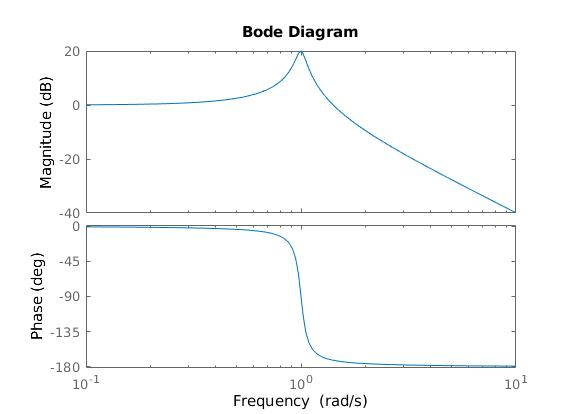
\includegraphics[width=\textwidth]{bode.jpg}
    \caption{Charakterystyka Bodego dla układu o transmitancji $K(s) = \frac{1}{s^2+0,1s+1}$}
\end{figure}

Z rozważań wynikło, że:
\begin{enumerate}
    \item kiedy $\omega = 0,1$, amplituda $A=1$ i przesunięcie fazowe $\varphi = 0 ^\circ$;
    \item kiedy $\omega = 1$, amplituda $A=10$ i przesunięcie fazowe $\varphi \approx 84,68 ^\circ$;
    \item kiedy $\omega = 10$, amplituda $A=0,1$ i przesunięcie fazowe $\varphi = 180 ^\circ$.
\end{enumerate}
Można zauważyć, że zgadza się to z amplitudą i przesunięciem fazowym ukazanym na charakterystyce Bodego:
\begin{enumerate}
    \item kiedy $\omega = 0,1$, amplituda $A=0 dB = 20\cdot log \frac{x}{1} = 1$ i przesunięcie fazowe $\varphi = 0 ^\circ$;
    \item kiedy $\omega = 1$, amplituda $A=20dB = 20\cdot log \frac{x}{1} = 10$ i przesunięcie fazowe $\varphi \approx -90^\circ$;
    \item kiedy $\omega = 10$, amplituda $A=-40 dB = 20\cdot log \frac{x}{1} = 0,1$ i przesunięcie fazowe $\varphi = -180 ^\circ$.
\end{enumerate}


\section{Badania w dziedzinie częstotliwościowej}
\subsection{Charakterystyka amplitudowo-fazowa}
\subsection{Analiza charakterystyki częstotliwościowej układu opóźniającego z inercją}

\section{Podsumowanie i wnioski}

\end{document}